\label{ssec:display}
For most people, especially people who do not deal with robots in their day-to-day life, interaction with robots is not as easy as one would like it to be. It is often diffuclt to hear what the robot is saying and it is not always intuitive for people to know when to talk to the robot. To remedy this, the head display of HERO is used. On this display that is integrated in the Toyota HSRs' `head', a lot of useful information can be displayed. Through the \emph{hero\_ display}\footnote{\url{https://github.com/tue-robotics/hero-display}} a few different functionalities are integrated. As per default, our Tech United @Home logo with a dynamic background is shown on the screen, as depicted in Figure \ref{fig:hero_display}. When the robot is speaking the spoken text is displayed, when the robot is listening a spinner along with an image of a microphone is shown and it is possible to display images.

\begin{figure}[h]
    \centering
	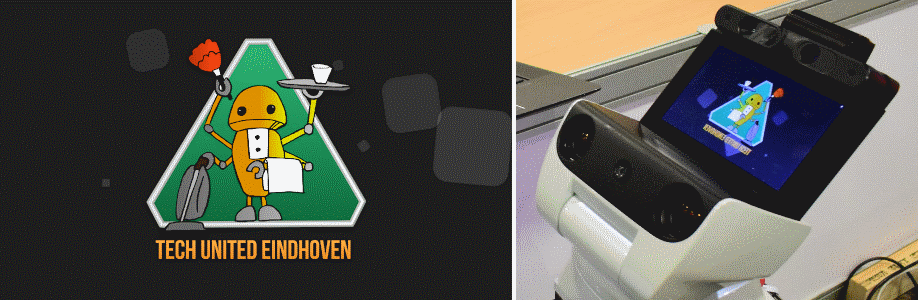
\includegraphics[width=\linewidth]{hero_display2}
    %\vspace{-0.5em}
	\caption{
		The default status of HERO's head display.}
	\label{fig:hero_display}
\end{figure}